%***********************************************************************
\subsection{Calibration Evaluation}\label{sub:bc_calibration_evaluation}
%***********************************************************************

% Opening Paragraph
The implication of the model parameters posterior uncertainty on the prediction is investigated by propagating the uncertainty through \gls[hyper=false]{trace} simulations of test No. $216$ (the calibration data) as well as the other five \gls[hyper=false]{feba} tests.
Samples of size $1'000$ are randomly picked directly from the joint posterior samples and are used to execute \gls[hyper=false]{trace} simulations.
Furthermore, the uncertainties related to the boundary conditions ($4$ additional parameters, namely \texttt{breakP}, \texttt{fillV}, \texttt{fillT}, and \texttt{pwr}) are also propagated alongside the posterior samples from each calibration scheme.  
Finally, for comparison purpose and for selected calibration schemes, the uncertainty propagation is also conducted without taking into account the correlation structure of the model parameters posterior uncertainties.
In other words, only the information from the posterior univariate marginals is used for the propagation and the parameters are considered independent of each other.

% Explaining the figure
Figs.~\ref{fig:ch5_plot_trace_uq_post_all_disc_tc_216}, \ref{fig:ch5_plot_trace_uq_post_all_disc_dp_216}, and~\ref{fig:ch5_plot_trace_uq_post_all_disc_co_216} show the propagation of the uncertainties for the clad temperature ($TC$), the pressure drop ($DP$), and the liquid carryover ($CO$) outputs, respectively.
The model parameters posterior uncertainties used in these figures are the ones obtained from the calibration scheme with model bias term and considering all types of output (i.e., \texttt{w/ Bias, All} in Table~\ref{tab:ch5_calibration_schemes}). 
The uncertainty bands correspond to the symmetric $95\%$ probability of the output uncertainties, i.e., the area between $2.5$-th and $97.5$-th percentiles of the outputs at each time step.
The dark gray band corresponds to the model parameters prior uncertainties propagation, while the two lighter bands correspond to the posterior uncertainties.
Two posterior uncertainties propagation results are presented, one (the lighter band) takes into account correlation structure of the posterior samples while the other one does not (i.e., independent samples).
This color convention will be used in all the other presentations of the uncertainty propagation results.
Finally, solid lines, dashed lines, and crosses correspond to the simulation with the nominal parameters values, the median of the posterior runs, and the experimental data, respectively.

% FEBA Test No. 216 Posterior w/ bias term Uncertainty Propagation, TC
\begin{sidewaysfigure}
	\centering
	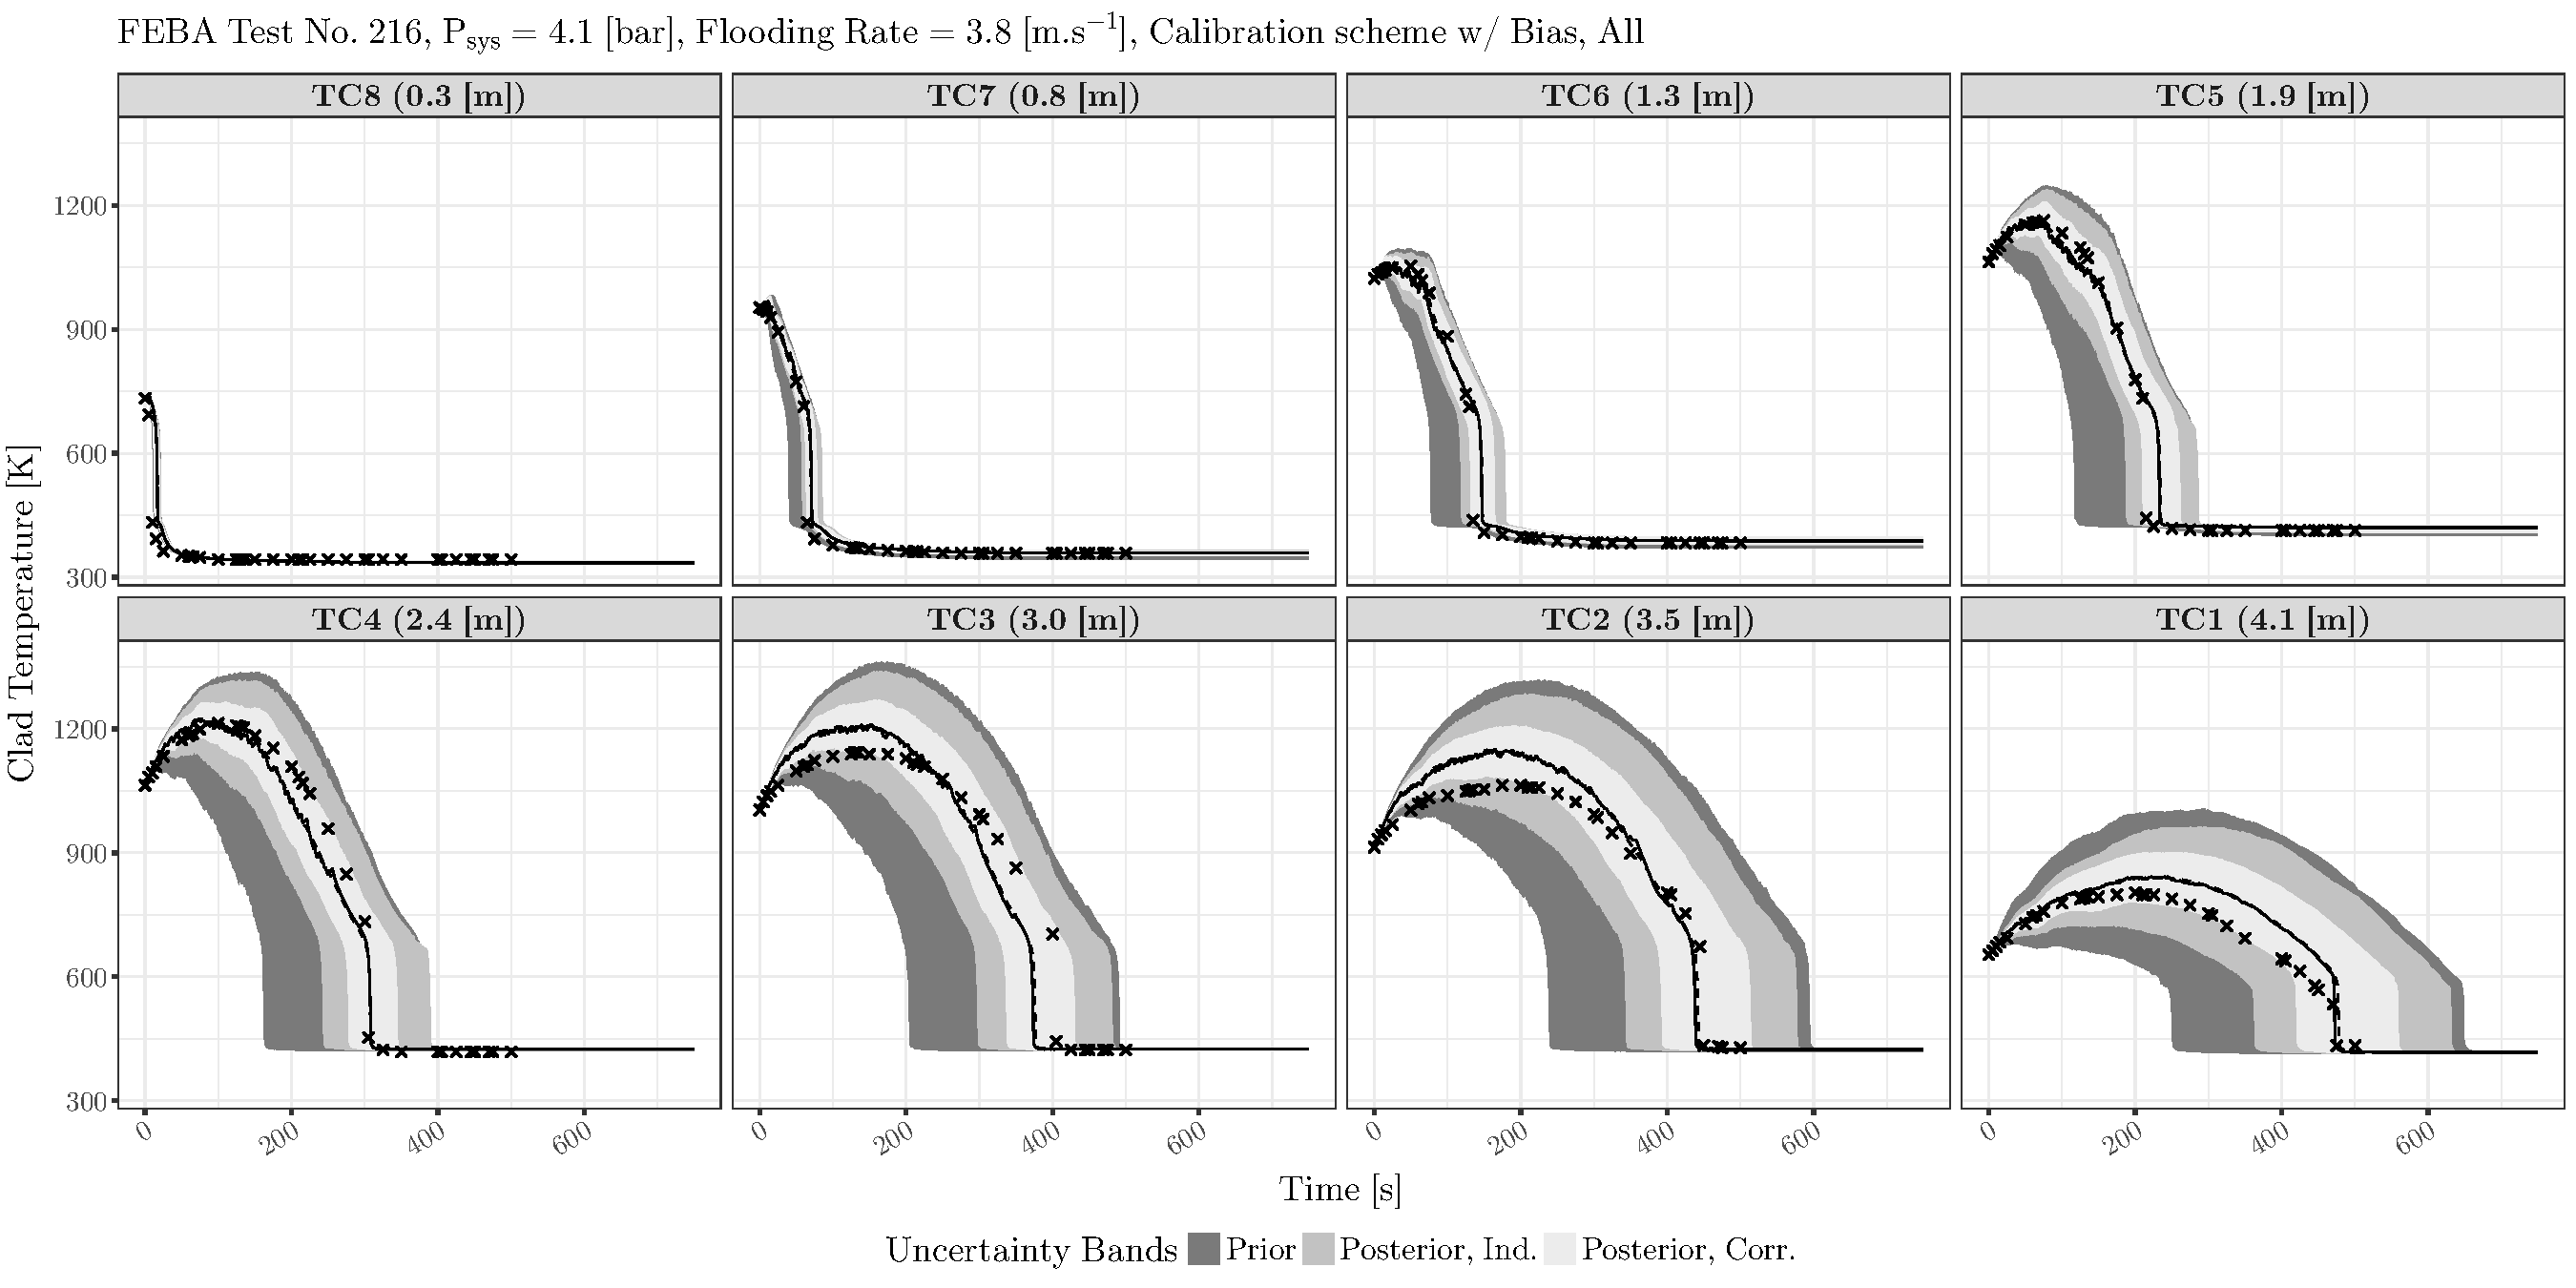
\includegraphics[width=0.90\textwidth]{../figures/chapter5/figures/plotTraceUQPosteriorAllDiscCenteredTC216}
		\captionof{figure}[Posterior uncertainty propagation of FEBA Test No. $216$ for the cladding temperature output ($TC$). The posterior samples are from the calibration scheme \texttt{w/ Bias, All}.]{Uncertainty propagation of the parameters uncertainty of \gls[hyper=false]{feba} Test No. $216$ for the cladding temperature output ($TC$) at different axial locations. The uncertainty bands refer to the symmetric $95\%$ probabilities. Solid lines, dashed lines, and crosses indicate the simulation with the nominal parameters values, the median of the posterior, and the experimental data, respectively. The posterior samples are from the calibration with model bias term and considering all types of output (\texttt{w/ Bias, All}).}
	\label{fig:ch5_plot_trace_uq_post_all_disc_tc_216}
\end{sidewaysfigure}

% Explaining the figure, TC
Fig.~\ref{fig:ch5_plot_trace_uq_post_all_disc_tc_216} shows the uncertainty propagation for the time-dependent $TC$ outputs at all axial levels with the posterior samples correspond to the calibration scheme \texttt{w/ Bias, All}.
As can be seen the posterior uncertainties of the clad temperature prediction are narrower as compared to the prior uncertainties across all axial elevation and at all time points.
All uncertainty bands, however, shows similar behavior regarding their inflation going from the bottom part of the assembly to the top of the assembly, and from the start of the transient to the time of quenching.
Furthermore, the median of the posterior predictions (dashed lines) coincides almost perfectly with the prediction of the nominal \gls[hyper=false]{trace} run (solid lines).

A comparison between the bands of correlated posterior samples and of independent posterior samples shows that the prediction uncertainties obtained using the correlated samples are much narrower and, at times, the experimental data points fall outside the uncertainty band.
However, the shape of the band looks consistent with the nominal run.
For instance, looking at the panel of $TC2$ in Fig.~\ref{fig:ch5_plot_trace_uq_post_all_disc_tc_216},
it can inferred that for the simulation to envelop the experimental data points in the early transient, it will also result in a reflood curve that increase the discrepancy even more in the later phase of the transient, especially near the time of quenching.
In other words, there is a certain ``rigidity'' associated with the \gls[hyper=false]{trace} reflood curve that cannot be arbitrarily bend.

On the other hand, not considering the correlation between model parameters in the posterior samples results in inflated uncertainties in the clad temperature prediction.
While the lower uncertainty bound for the independent samples is much narrower than that of the prior, the upper uncertainty bound is closer to the upper uncertainty bound than that of the prior.

% FEBA Test No. 216 Posterior w/ bias term Uncertainty Propagation, DP
Fig.~\ref{fig:ch5_plot_trace_uq_post_all_disc_dp_216} shows the uncertainty propagation for the time-dependent $DP$ outputs for each of the axial segments.
The posterior samples correspond to the calibration scheme \texttt{w/ Bias, All}.
Once again the posterior uncertainties propagation result in narrower uncertainty bands as compared to that with the prior across all axial segments and all time points.
However, the difference between taking and not taking into account correlation between model parameters is less striking for this type of output.
Moreover, all uncertainty bands cover most of the experimental data.
\bigfigure[pos=tbhp,
           opt={width=1.0\textwidth},
           label={fig:ch5_plot_trace_uq_post_all_disc_dp_216},
           shortcaption={Posterior uncertainty propagation of FEBA Test No. $216$ for the pressure drop output ($DP$). The posterior samples are from the calibration scheme \texttt{w/ Bias, All}.}]
{../figures/chapter5/figures/plotTraceUQPosteriorAllDiscCenteredDP216}
{Uncertainty propagation of the parameters uncertainty of \gls[hyper=false]{feba} Test No. $216$ for the pressure drop output ($DP$) at different axial segments. The uncertainty bands refer to the symmetric $95\%$ probabilities. Solid lines, dashed lines, and crosses indicate the simulation with the nominal parameters values, the median of the posterior, and the experimental data, respectively. The posterior samples are from the calibration scheme \texttt{w/ Bias, All}.}

% FEBA Test No. 216 Posterior w/ bias term Uncertainty Propagation, CO
Fig.~\ref{fig:ch5_plot_trace_uq_post_all_disc_co_216} shows the propagation for the time-dependent $CO$ output up to the saturation of the measurement tank at $10 [kg]$ with the posterior samples correspond to the calibration scheme \texttt{w/ Bias, All}.
Unlike the previous two types of output, the nominal \gls[hyper=false]{trace} prediction exhibits large bias compared to the experimental data.
While the large prior uncertainty manages to cover the experimental data points, all of the points fall outside the posterior uncertainty bounds both with and without taking into account correlation among parameters.
As the calibration scheme \texttt{w/ Bias, All} simultaneously takes into account the three types of output, and considering the results of uncertainty propagation for the two other outputs, it can be inferred that this failure to cover the experimental data points is off-set by the more consistent bands for the other two outputs.
\begin{figure}[!bth]
    \centering
    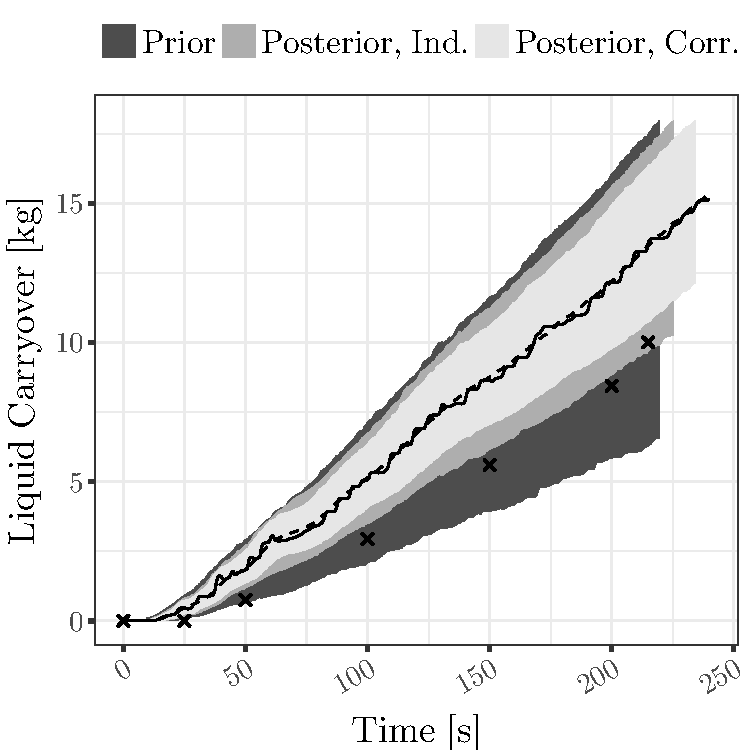
\includegraphics[width=0.5\textwidth]{../figures/chapter5/figures/plotTraceUQPosteriorAllDiscCenteredCO216}
    \caption[Posterior uncertainty propagation of FEBA Test No. $216$ for the liquid carryover output ($CO$). The posterior samples are from the calibration scheme \texttt{w/ Bias, All}.]{Uncertainty propagation of the parameters uncertainty of \gls[hyper=false]{feba} Test No. $216$ for the liquid carryover output ($CO$). The uncertainty bands refer to the symmetric $95\%$ probabilities. Solid lines, dashed lines, and crosses indicate the simulation with the nominal parameters values, the median of the posterior, and the experimental data, respectively. The posterior samples are from the calibration scheme \texttt{w/ Bias, All}.}
    \label{fig:ch5_plot_trace_uq_post_all_disc_co_216}
\end{figure}

% Calibration Score vs Informativeness
Instead of showing similar plots of the uncertainty propagation to present the effect of different posterior samples obtained from different calibration schemes on the other \gls[hyper=false]{feba} tests, Fig.~\ref{fig:ch5_plot_calib_info} is used to summarize the effect on the uncertainty propagation in a single plot using the concepts of \emph{calibration score} and \emph{informativeness} previously explained (see Section~\ref{sub:bc_simulation_experiment} and Appendix~\ref{app:calib_info}).
The plots like Figs.~\ref{fig:ch5_plot_trace_uq_post_all_disc_tc_216}, \ref{fig:ch5_plot_trace_uq_post_all_disc_dp_216}, and~\ref{fig:ch5_plot_trace_uq_post_all_disc_co_216} for all the other cases corresponding to different \gls[hyper=false]{feba} tests and calibration schemes are available in Appendix~\ref{app:mcmc_evaluation} for reference.

% How to read the plot
Fig.~\ref{fig:ch5_plot_calib_info} presents the calibration score vs. informativeness for different \gls[hyper=false]{feba} tests, different calibration schemes, and different types of outputs (clad temperature $TC$, pressure drop $DP$, and liquid carryover $CO$).
In each panel, the vertical lines correspond to the initial informativeness, that is, that of the prior.
This initial informativeness are taken to be zero uniformly across output types and \gls[hyper=false]{feba} tests as it represents the widest uncertainty band considered.
The horizontal lines, on the other hand, correspond to the initial calibration score of the prior uncertainty bands and the nominal \gls[hyper=false]{trace} run as its reference simulation value.
As can be seen the scores are slightly different from test to test and from output type to output type.
Finally, the results of propagating posterior samples obtained from each calibration scheme to the \gls[hyper=false]{trace} \gls[hyper=false]{feba} model in terms of calibration score and informativeness are plotted.
In each panel, going from left to right indicates the narrowing of uncertainty band and the increase of informativeness and vice versa;
while going from bottom to top indicates the closer the prediction and its uncertainty to the experimental data.

\clearpage
\begin{sidewaysfigure}
	\centering
	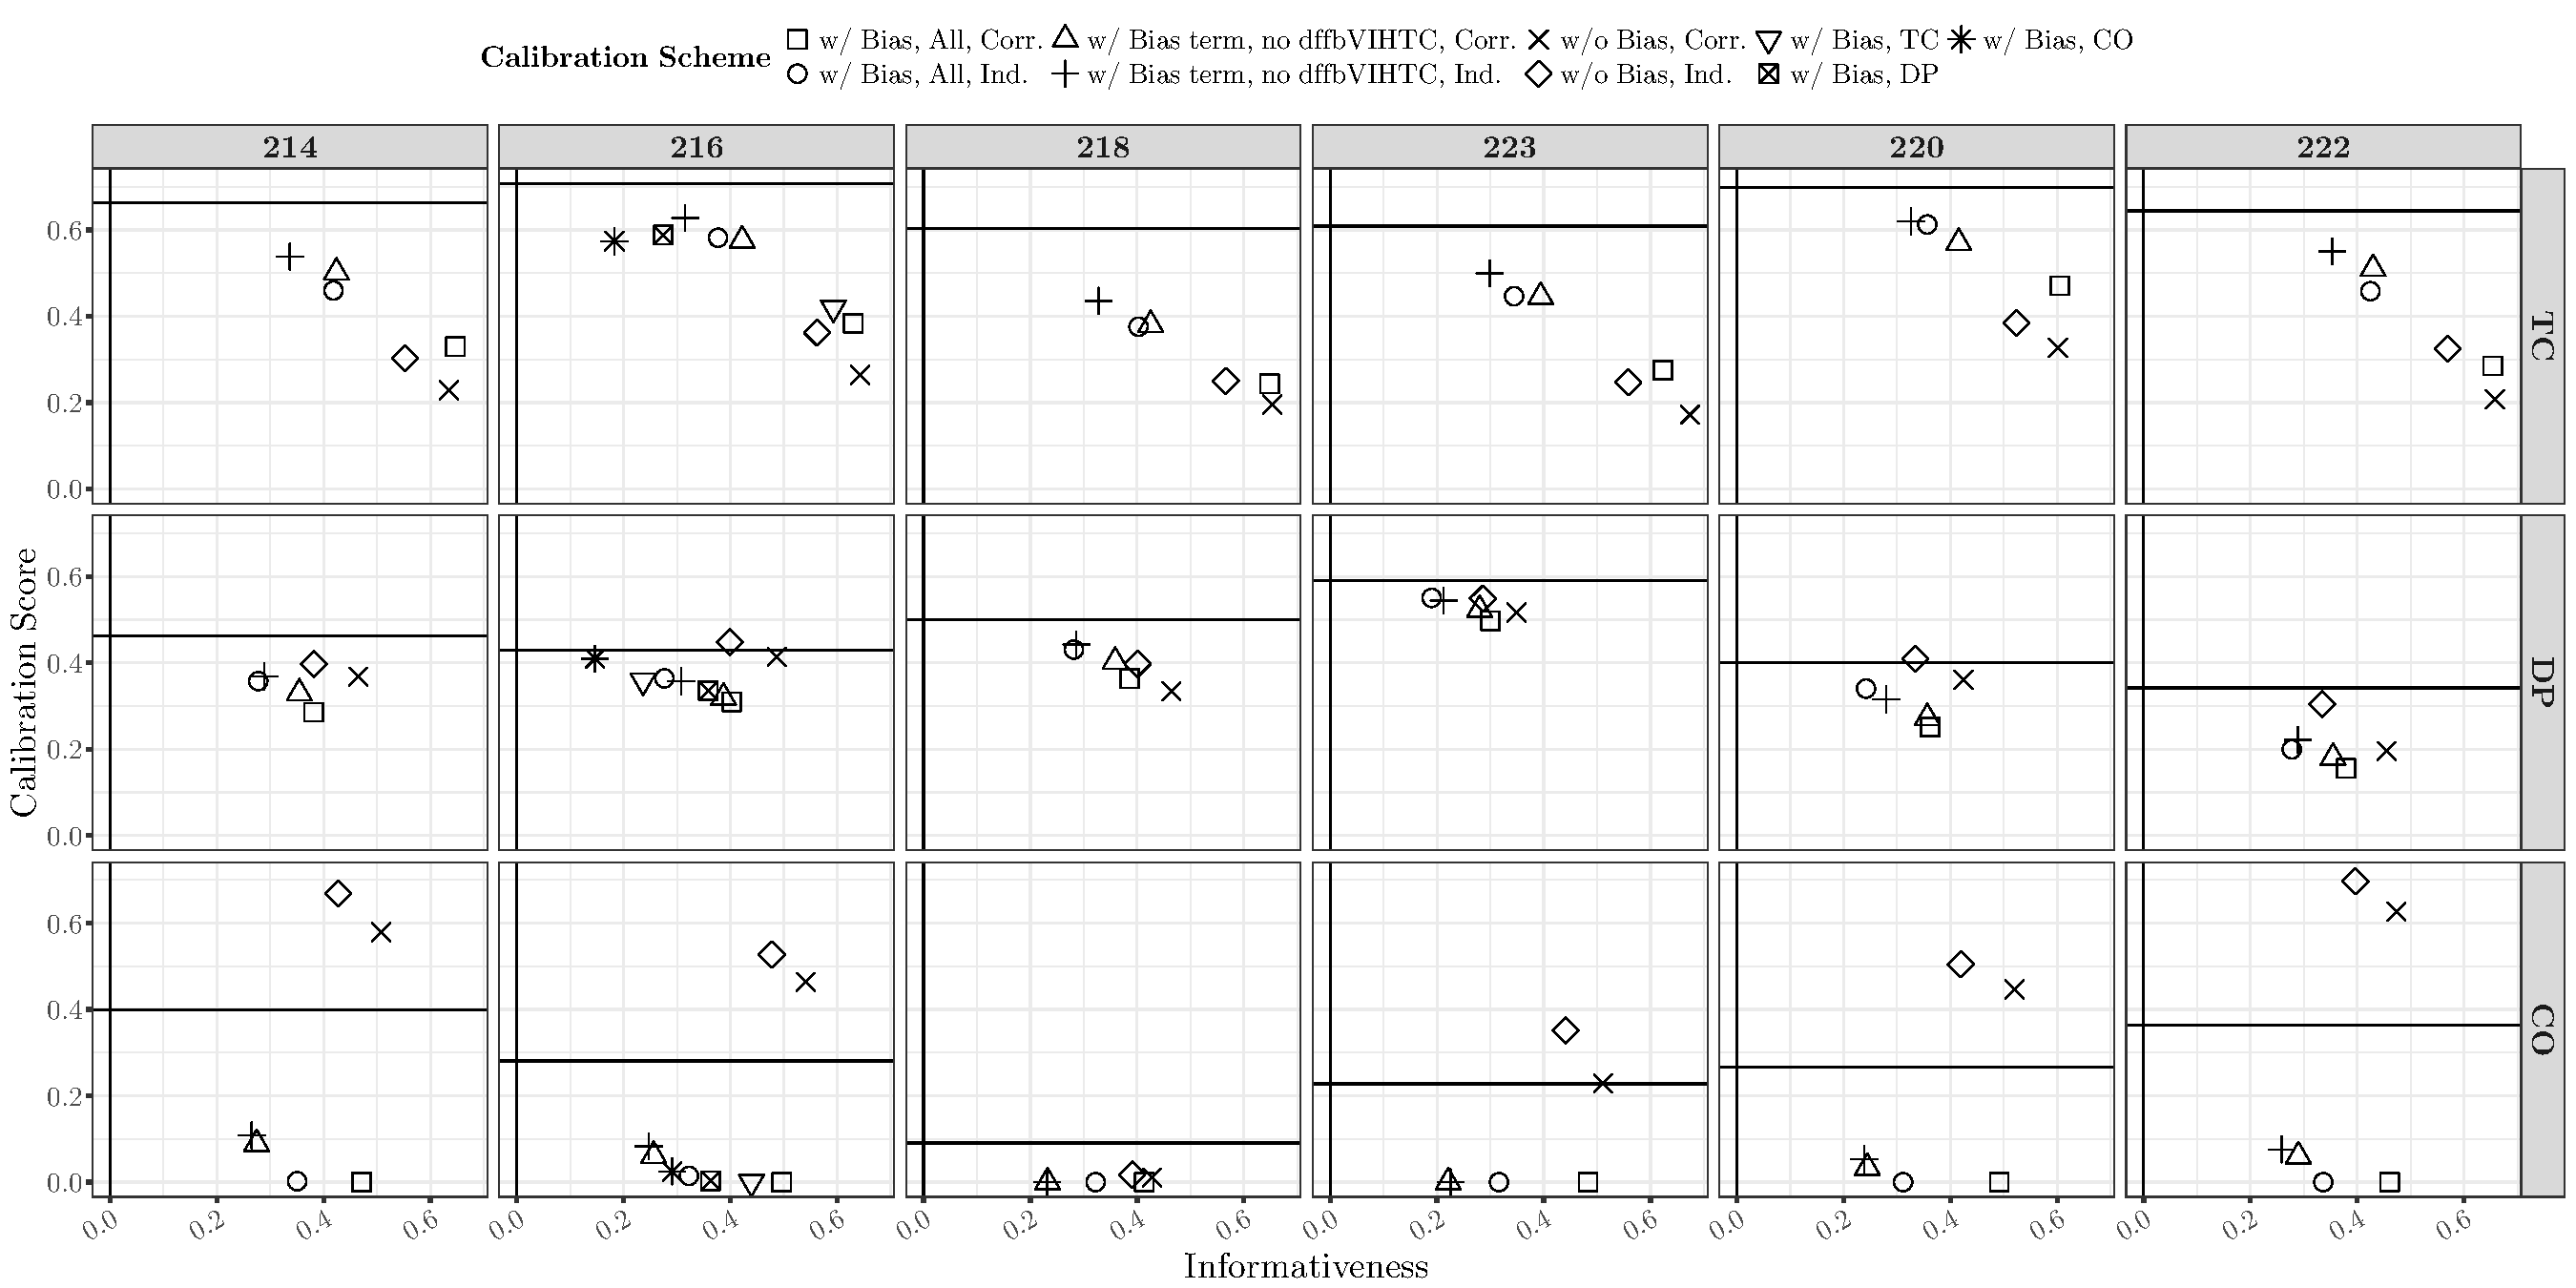
\includegraphics[width=0.95\textwidth]{../figures/chapter5/figures/plotCalibInfo}
		\captionof{figure}[Calibration score vs. Informativeness for different posterior samples propagated on all the FEBA tests.]{Calibration score vs. Informativeness for different posterior samples propagated on all the \gls[hyper=false]{feba} tests. Vertical lines indicate the informativeness of the prior uncertainty (defined as $0$) while the horizontal lines indicate the initial Calibration score (i.e., that of the prior).}
	\label{fig:ch5_plot_calib_info}
\end{sidewaysfigure}
\clearpage

% Comparing Results, calibration scheme
For the $TC$ output, and except for the \gls[hyper=false]{feba} test No. $216$ (the calibration data), there is an apparent linear relationship between calibration score and informativeness.
That is the propagation that results in the narrowest uncertainty band (high informativeness) tends to have higher failure in enveloping the experimental data (low calibration score).
Recall that a failure in enveloping experimental data point is assigned to have a zero calibration score.
The results of the scheme \texttt{w/o Bias}, in particular, have the lowest calibration score with respect to the $TC$ output while at the same time score high in the informativeness. 
On the other hand, for the same level of informativeness, the results of the scheme \texttt{w/ Bias, All} have higher calibration scores across all the \gls[hyper=false]{feba} tests.

This relationship does not present with respect to the $DP$ output.
There the calibration scores for all the calibration schemes fall near the initial calibration score, while having higher informativeness.
Furthermore, except for the propagation the \gls[hyper=false]{feba} test No. $216$ there is not so much variation in the informativeness; the points tend to cluster together especially in comparison with that of the $TC$.

Finally, most calibration schemes results in much lower calibration score with respect to the $CO$ output, some even fall to zero.
That is, the resulting uncertainty bands completely fail to envelop a single experimental data points.
At the same time, the results of the scheme \texttt{w/o Bias} manage to improve the prediction on the output, both in terms of calibration score and informativeness; the results are better compared to that of the prior.

% Comparing Results, correlated vs independent posterior samples
Considering correlation between the model parameters in the propagation affects the calibration score and the informativeness.
Taking into account the correlation in the propagation is consistently increasing the informativeness (tightening the uncertainty band) while simultaneously lowering the calibration score across all the \gls[hyper=false]{feba} tests.
On the contrary, taking the model parameters to be independent of each other deflates the informativeness (widen the uncertainty band) while simultaneously increases the calibration score.
The effect can be observed across outputs, calibration schemes, and \gls[hyper=false]{feba} tests; though it is especially strong for the scheme \texttt{w/ Bias, All} and for the $TC$ output, while the effect is more marginal for the other schemes and output types.

% Comparing Results, between FEBA Tests
Comparing the results between different \gls[hyper=false]{feba} tests some interesting observations can be made.
The informativeness and the calibration score for all the calibration schemes seem to fall relatively at the same position for each of the \gls[hyper=false]{feba} tests.
Though the calibration scores relative positions varies slightly across different \gls[hyper=false]{feba} tests,
the maximum informativeness with respect to the $TC$, $DP$, $CO$ outputs are $0.7$, $0.5$, $0.5$, respectively, for all the \gls[hyper=false]{feba} tests.
This indicates that the uncertainty band in the prediction due to the posterior uncertainties (obtained on the basis of a single test) are relatively insensitive to boundary conditions of the tests.
It is only for the $CO$ output \gls[hyper=false]{feba} test No. 218, no calibration scheme (not even \texttt{w/o Bias}) gives an improvement on the calibration score.

% Comparing results, different output for FEBA Test 216
Lastly, when comparing the effect of using different types of output in the calibration, and only for \gls[hyper=false]{feba} test No. $216$, it is shown considering all types of outputs increase informativeness in the prediction.
As expected, using any particular type of output causes the informativeness with respect to the other outputs to be low.
Moreover, the increase in informativeness from taking into account multiple type of outputs is not followed by large decrease of calibration score.
This is especially the case for the $DP$ (and $TC$) output where the improvement on the informativeness is significant when compared to the results of calibration using experimental data other than the $DP$ (and $TC$, respectively) itself.
This gives an indication that the model parameters responsible for the improvement with respect to each output might be different as was previously showed by sensitivity analysis.
Curiously this is not the case for the $CO$ output as the calibration using only the $CO$ experimental data gives lower informativeness compared to the calibration using the other types of data.